%-------------------------------------------------------------------------------
%	The MIT License (MIT)
%
%	Copyright (c) 2025 - Today Jan Küster <info@jankuester.com>
%
%	https://github.com/jankapunkt/latexcv
%
%	Permission is hereby granted, free of charge, to any person obtaining a copy
%	of this software and associated documentation files (the "Software"), to deal
%	in the Software without restriction, including without limitation the rights
%	to use, copy, modify, merge, publish, distribute, sublicense, and/or sell
%	copies of the Software, and to permit persons to whom the Software is
%	furnished to do so, subject to the following conditions:
%	
%	THE SOFTWARE IS PROVIDED "AS IS", WITHOUT WARRANTY OF ANY KIND, EXPRESS OR
%	IMPLIED, INCLUDING BUT NOT LIMITED TO THE WARRANTIES OF MERCHANTABILITY,
%	FITNESS FOR A PARTICULAR PURPOSE AND NONINFRINGEMENT. IN NO EVENT SHALL THE
%	AUTHORS OR COPYRIGHT HOLDERS BE LIABLE FOR ANY CLAIM, DAMAGES OR OTHER
%	LIABILITY, WHETHER IN AN ACTION OF CONTRACT, TORT OR OTHERWISE, ARISING FROM,
%	OUT OF OR IN CONNECTION WITH THE SOFTWARE OR THE USE OR OTHER DEALINGS IN
%	THE SOFTWARE.
%	
%
%-------------------------------------------------------------------------------


%============================================================================%
%
%	DOCUMENT DEFINITION
%
%============================================================================%
% we use article class because we want to fully customize the page 
% and thus, do not use a CV template
\documentclass[10pt,A4]{article}


%----------------------------------------------------------------------------------------
%	ENCODING
%----------------------------------------------------------------------------------------
% we use utf8 since we want to build from any machine
\usepackage[utf8]{inputenc}

%----------------------------------------------------------------------------------------
%	LOGIC
%----------------------------------------------------------------------------------------
% provides \isempty test
\usepackage{xifthen}

%----------------------------------------------------------------------------------------
%	FONT
%----------------------------------------------------------------------------------------
% some tex-live fonts - choose your own

% \usepackage[defaultsans]{droidsans}
% \usepackage[default]{comfortaa}
% \usepackage{cmbright}
% \usepackage[default]{raleway}
% \usepackage{fetamont}
% \usepackage[default]{gillius}
% \usepackage[light,math]{iwona}
\usepackage[default]{roboto} 

% set font default
\renewcommand*\familydefault{\sfdefault} 	
\linespread{1.22}

\usepackage[T1]{fontenc}

% more font size definitions
\usepackage{moresize}

% use icons as fonts
\usepackage{fontawesome5}


%----------------------------------------------------------------------------------------
%	PAGE LAYOUT  DEFINITIONS
%----------------------------------------------------------------------------------------
% debug page outer frames
% \usepackage{showframe}			

% define page styles using geometry,
% so you can adjust page margins, if desired
% \usepackage[a4paper]{geometry}		
% \geometry{top=1.25cm, bottom=-.6cm, left=1.5cm, right=1.5cm} 	

% use customized header
\usepackage{fancyhdr}				
\pagestyle{fancy}

% less space between header and content
\setlength{\headheight}{-5pt}


% customize entries left, center and right
% \lhead{}
% \chead{}
% \rhead{}


% new paragraph indentation is zero
\setlength{\parindent}{0mm}

%----------------------------------------------------------------------------------------
%	TABLE /ARRAY DEFINITIONS
%---------------------------------------------------------------------------------------- 

% for layouting tables
\usepackage{multicol}			
\usepackage{multirow}

% extended aligning of tabular cells
\usepackage{array}

\newcolumntype{x}[1]{%
>{\raggedleft\hspace{0pt}}p{#1}}%


%----------------------------------------------------------------------------------------
%	GRAPHICS DEFINITIONS
%---------------------------------------------------------------------------------------- 

% for header image
\usepackage{xcolor,graphicx}
% for more controlled boxes with bg colors, borders etc.
\usepackage[many]{tcolorbox}

% for floating figures
\usepackage{wrapfig}
\usepackage{float}
% \floatstyle{boxed} 
% \restylefloat{figure}

% for drawing graphics		
% \usepackage{tikz}				
% \usetikzlibrary{shapes, backgrounds,mindmap, trees}

%----------------------------------------------------------------------------------------
%	LINKS / URLS
%---------------------------------------------------------------------------------------- 
%Package for links, must be the last package used
\usepackage[hidelinks]{hyperref}

\newcommand{\link}[1]{\textcolor{bgcol}{\href{#1}{#1}}}

%----------------------------------------------------------------------------------------
%	Color DEFINITIONS
%---------------------------------------------------------------------------------------- 

\usepackage{color}

% accent color
\definecolor{sectcol}{RGB}{150,200,0}

% dark background color
\definecolor{bgcol}{RGB}{110,110,110}

% light background / accent color
\definecolor{softcol}{RGB}{225,225,225}


%============================================================================%
%
%
%	DEFINITIONS
%
%
%============================================================================%

%----------------------------------------------------------------------------------------
% 	HEADER
%----------------------------------------------------------------------------------------

% remove top header line
\renewcommand{\headrulewidth}{0pt} 

% remove bottom header line
\renewcommand{\footrulewidth}{0pt}	  	

% remove pagenum
\renewcommand{\thepage}{}	

% remove section num		
\renewcommand{\thesection}{}			

%----------------------------------------------------------------------------------------
% 	ARROW GRAPHICS in Tikz
%----------------------------------------------------------------------------------------

% a six pointed arrow pointing to the left
\newcommand{\tzlarrow}{(0,0) -- (0.2,0) -- (0.3,0.2) -- (0.2,0.4) -- (0,0.4) -- (0.1,0.2) -- cycle;}	

% include the left arrow into a tikz picture
% param1: fill color
%
\newcommand{\larrow}[1]
{\begin{tikzpicture}[scale=0.58]
	 \filldraw[fill=#1!100,draw=#1!100!black]  \tzlarrow
 \end{tikzpicture}
}

% a six pointed arrow pointing to the right
\newcommand{\tzrarrow}{ (0,0.2) -- (0.1,0) -- (0.3,0) -- (0.2,0.2) -- (0.3,0.4) -- (0.1,0.4) -- cycle;}

% include the right arrow into a tikz picture
% param1: fill color
%
\newcommand{\rarrow}
{
\begin{tikzpicture}[scale=0.7]
	\filldraw[fill=sectcol!100,draw=sectcol!100!black] \tzrarrow
 \end{tikzpicture}
}



%----------------------------------------------------------------------------------------
%	custom sections
%----------------------------------------------------------------------------------------

% create a coloured box with arrow and title as cv section headline
% param 1: section title
%
\newcommand{\cvsection}[1]
{
	\begin{flushleft}
		\LARGE\textcolor{black}{\uppercase{#1}}	\\[20pt]
	\end{flushleft}
}

%----------------------------------------------------------------------------------------
%	 CV EVENT
%----------------------------------------------------------------------------------------

% creates a stretched box as cv entry headline followed by some paragraphs about 
% the work you did
% uses vbox, which is never broken across pages!
% param 1:	event time i.e. 2014 or 2011-2014 etc.
% param 2:	event name (what did you do?)
% param 3:	institution (where did you work / study)
% param 4:	list of paragraphs
%
\newcommand{\cvevent}[4] {
\begin{flushleft}
\vbox{
\textcolor{sectcol}{\textbf{#2}}\\
\textcolor{bgcol}{{#3} | {#1}}\\[10pt]
}
\foreach \desc in {#4}{\vbox{\desc\\[10pt]}}
\end{flushleft}
\vspace{10pt}
}

%----------------------------------------------------------------------------------------
% CUSTOM STRUT FOR EMPTY BOXES
%----------------------------------------- -----------------------------------------------
\newcommand{\mystrut}{\rule[-.3\baselineskip]{0pt}{\baselineskip}}

%----------------------------------------------------------------------------------------
% CUSTOM LOREM IPSUM
%----------------------------------------------------------------------------------------
\newcommand{\lorem}
{Lorem ipsum dolor sit amet, consectetur adipiscing elit. Donec a diam lectus.}

%----------------------------------------------------------------------------------------
%	ICON-SET EMBEDDING
%---------------------------------------------------------------------------------------- 

% font awesome icon
\newcommand{\icon}[1]{\makebox[10pt][c]{\textcolor{sectcol}{\csname fa#1\endcsname}}}

%icon with text shortcut
\newcommand{\icontext}[2]{
	\icon{#1} \small{#2}
}

%============================================================================%
%
%
%
%	DOCUMENT CONTENT
%
%
%
%============================================================================%
\begin{document}


% use our custom fancy header definitions
\pagestyle{fancy}	


%----------------------------------------------------------------------------------------
%	HEADER IMAGE
%----------------------------------------------------------------------------------------
\begin{figure}[H]
\begin{center}
	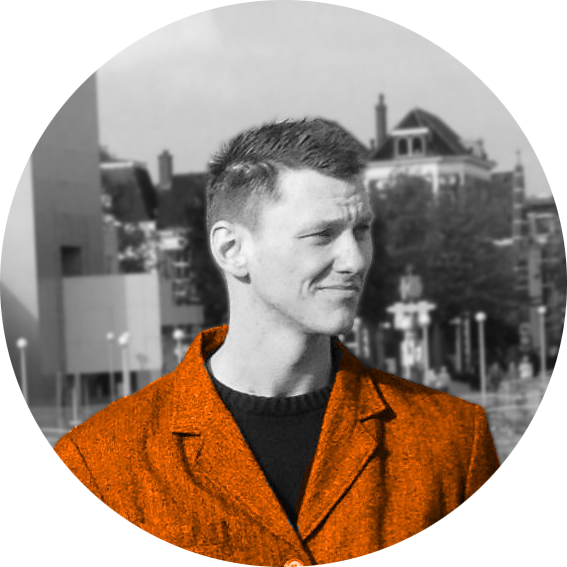
\includegraphics[width=0.4\linewidth]{myfoto.png}
\end{center}
\end{figure}

%---------------------------------------------------------------------------------------
%	TITLE HEADLINE
%----------------------------------------------------------------------------------------
\vspace{-48pt}
\textcolor{softcol}{\hrule}
\colorbox{white}{\makebox[1\linewidth][c]{
	\HUGE \textsc{Jan Küster} \textcolor{sectcol}{\rule[-1mm]{1mm}{0.9cm}} \textsc{M.Sc.}
}}

\begin{center}
	\small \textsc{Research Software Engineer}
\end{center}




%---------------------------------------------------------------------------------------
%	META SECTION
%----------------------------------------------------------------------------------------
\begin{center}
\icontext{MapMarker}{Bremen, Germany}
\href{mailto:info@jankuester.com}{\icontext{Envelope}{info@jankuester.com}}
\icontext{Mobile}{+49 170 123 456 789}
\\[10pt]
\href{https://jankuester.com}{\icontext{MousePointer}{jankuester.com}}
\href{https://github.com/jankapunkt}{\icontext{Github}{github.com/jankapunkt}}
\href{https://orcid.org/0009-0008-8088-9837}{\icontext{Orcid}{0009-0008-8088-9837}}
\end{center}

\normalsize

%---------------------------------------------------------------------------------------
%	SUMMARY (optional)
%----------------------------------------------------------------------------------------
\textcolor{softcol}{\hrule}
\bigskip

I am a Digital Media graduate with 10+ years of experience as research software engineer.
My main focus is on production-grade web applications, involving real world users for
long-term evaluations in the field.
For this I leverage primarily web standards, as well as available modern web-technologies.

%============================================================================%
%
%	CV SECTIONS AND EVENTS (MAIN CONTENT)
%
%============================================================================%

%---------------------------------------------------------------------------------------
%	PUBLICATIONS
%----------------------------------------------------------------------------------------
\cvsection{Publications}

\vbox{
Belli, A., Küster, J., Matayeva, L., Hohmann, F., Sinner, P., Krüger, G., Wolf, K., \& Hepp, A. (2025). OpenQDA (1.0.0). 
Zenodo.\\
\link{https://doi.org/10.5281/zenodo.14772936}\\
}

\vbox{
Küster, J. (2024, March 6). Software Applications for Individuals with Low Literacy - Key Insights and Takeaways in Research Software Engineering from an Interdisciplinary Project.
4th conference for Research Software Engineering in Germany (deRSE24), Julius-Maximilians-Universität Würzburg. Zenodo.\\
\link{https://doi.org/10.5281/zenodo.10810074}\\
}

\vbox{
Küster, J., Meyer, I. A. M., Windler, M., Karsten D. Wolf, \& Koppel, I. (2023). 
leaonline/leaonline-app: 1.1.0 (v1.1.0). Zenodo.\\
\link{https://doi.org/10.5281/zenodo.10816689}
}
%---------------------------------------------------------------------------------------
%	CODE
%----------------------------------------------------------------------------------------
\newpage
\cvsection{Relevant Repositories}

OpenQDA - \link{https://github.com/openqda}

lea.Online - \link{https://github.com/leaonline}

Node OAuth - \link{https://github.com/node-oauth}

%---------------------------------------------------------------------------------------
%	EXPERIENCE
%----------------------------------------------------------------------------------------
\bigskip
\cvsection{Research Projects}

\cvevent{2023 - Today}{OpenQDA - A Free Sustainable Qualitative Research Software}{ZeMKI, University of Bremen}{
	{Goal: Develop a free and alternative to commercial QDA software},
	{Key responsibilities: System architecture, software design, (web-) client architecture and dependencies management.},
   {Major activity: Frontend implementation of rich interactive UI for qualitative data analysis using Vue3, Vite and TailwindCss.},
	{Secondary activities: Managing Github repositories, documentation, CI, code quality assurance.},
	{Available via \link{https://openqda.org}}
}

\cvevent{2023 - 2025}{IMPACT}{University of Bremen}{
	{Goal: Implement AI-based services as key tools in formative and summative assessment activities at the University of Bremen},
	{Key responsibilities: System architecture, software design, infrastructure, legal implications, GDPR, ethical considerations, requirements engineering},
   {Major activities: Requirements engineering and consulting},
	{Secondary activities: AI tool development using Python and respective libraries}
}

\cvevent{2019 - 2023}{lea.online}{University of Bremen}{
	{Goals: Develop a multi-application system to allow diagnostics and learning of adults with low literacy},
	{Key responsibilities: System architecture, software design, infrastructure, legal implications, GDPR, ethical considerations, outsourcing development, requirements engineering},
   {Major activities: web-app development, mobile app development (react native + expo)},
	{Secondary activities: GitHub repository management and maintenance},
	{Publications:},
	{Meyer, I. A. M., Wolf, K. D., Windler, M., \& Küster, J. (2024). Digitale berufsfeldbezogene Förderung von Literalität und Numeralität in der arbeitsorientierten Grundbildung mit der lea.App. In K.-H. Gerholz, S. Annen, R. Braches-Chyrek, J. Hufnagl, \& A. Wagner (Eds.), bwp@ Spezial HT2023 Fachkräftesicherung – Zukunftsweisende Qualifierziung, gesellschaftliche Teilhabe und Integration durch berufliche Bildung.\\ \link{https://www.bwpat.de/ausgabe/spezial-ht2023/meyer-etal}}
}

\cvevent{2016 - 2019}{CARO - Care Reflexion Online}{University of Bremen}{
	{Goals: Develop and evaluate a interactionistic classroom management system for German nursing education using \href{https://meteor.com}{MeteorJS}.},
	{Key responsibilities: System architecture, software Design, (web-) client architecture and dependencies management.},
   {Major activity: Fullstack implementation of entire software},
	{Secondary activities: Managing Github repositories, documentation, CI, code quality assurance.},
	{Publications:},
	{Darmann-Finck, I., Wolf, K. D., Schepers, C., \& Küster, J. (2021). Digital unterstütztes Lernen in der Pflegeausbildung: Die Care Reflection Online (CARO) – Lernumgebung. MedienPädagogik: Zeitschrift Für Theorie Und Praxis Der Medienbildung, 317–345.\\ \link{https://doi.org/10.21240/mpaed/jb16/2021.04.30.X}\\[10pt]}
	{Schepers, C., \& Küster, J. (2020). Sind Pflegeschulen bereit für den Einsatz digitaler Lehr-Lernformate? Berufsbildung, 181. \link{https://www.zeitschrift-berufsbildung.de/archiv/74-care-work-4-0}},
   {Project blog: \link{https://blogs.uni-bremen.de/caroprojekt/} (German)}
}

%
\cvevent{2012 - 2014}{DomPL-IK}{University of Bremen, part time}{
	{Invented a flexible assessment framework, targeting industrial trainees},
	{Supervised software development lifecycle, Recruited team members},
		{Publications:},
	{
	Seifried,J., Rausch,A., Kögler,K., Brandt,S., Eigenmann,R., Schley,T., Siegfried,C., Egloffstein, M., Küster,J., Wuttke,E., Sembill,D., Martens,T., Wolf,K.D. (2016). Problemlösekompetenz angehender Industriekaufleute – Konzeption des Messinstruments und ausgewählte empirische Befunde (DomPL-IK). In K. Beck/M. Landenberger/F. Oser (Hrsg.): Technologiebasierte Kompetenzmessung in der beruflichen Bildung – Ergebnisse aus der BMBF-Förderinitiative ASCOT. Bielefeld:WBV, 119-138 
	}
}

% \textcolor{softcol}{\hrule}

%
\cvevent{2011 / 11}{Project Management Simulation Training}{Getoq Consulting}{
	{Performed a two-day project simulation from management perspective},
	{Topics included customer contracts, change management, controlling, operational tasks}
}

% \textcolor{softcol}{\hrule}


%
\cvevent{2010 - 2011}{Student Assistant / Programmer}{University of Bremen}{
	{Realized an online diagnosis platform for workforce literacy development (Flex)},
	{Modeled software design, implemented various prototypes, conducted usability tests},
	{Publications:},
	{Koppel, I., Küster, J., \& Wolf, K. D. (2013). Usability testing with female functional illiterates,Usability-testing mit funktionalen analphabetinnen. Lecture Notes in Informatics (LNI), DEFLI Proceedings - Series of the Gesellschaft Für Informatik (GI), P-218, 293–296.}
}


%---------------------------------------------------------------------------------------
%	EDUCATION SECTION
%--------------------------------------------------------------------------------------
\bigskip
\cvsection{Education}

\cvevent{2015 / 07}{Graduated as M.Sc. Digital Media}{University of Bremen}{
	{Master Thesis: Semi Automated Scoring in Technology Based Assessment},
	{Developed and evaluated an algorithm for semi automated scoring of spreadsheet data}
}

% \textcolor{softcol}{\hrule}

%
\cvevent{2012 - 2013}{Master Project - PrIMA}{University of Bremen}{
	{Co-Invented a touch table application for medical support, co-developed software (Java)},
	{Formed a scrum team, mainted project dev server (Debian), surveyed target audience}
}

% \textcolor{softcol}{\hrule}

%
\cvevent{2012 - 2015}{Master Studies Digital Media}{University of Bremen}{
	{Inter-cultural classes in English, covering special topics in computer science and design},
	{Professionalized in research methods, software development and e-assessment}
}

% \textcolor{softcol}{\hrule}

%
\cvevent{2009 - 2010}{Semester Abroad}{University of Melbourne}{
	{Mastered six months of study and trans-cultural experience in Melbourne, Australia},
	{Finished machine programming, information visualization, professional essay writing}
}
\cvevent{2007 - 2011}{Bachelor Studies Digital Media}{University of Bremen}{
	{Foundations of Digial Media, Computer Science and Software Engineering}
}

%--------------------------------------------------------------------------------------------------
%	ARTIFICIAL FOOTER (fancy footer cannot exceed linewidth) 
%--------------------------------------------------------------------------------------------------

\null
\vspace*{\fill}
\hspace{-0.25\linewidth}\colorbox{white}{\makebox[1.5\linewidth][c]{\mystrut  \textnormal{\textcolor{sectcol}{https://jankuester.com} $\cdot$ \textcolor{sectcol}{github.com/jankapunkt}}}}




%============================================================================%
%
%
%
%	DOCUMENT END
%
%
%
%============================================================================%
\end{document}
